\documentclass[20pt]{article}
\usepackage[latin1]{inputenc}
\usepackage{epsf}
\usepackage{graphicx,psfrag,color,pstcol,pst-grad}
\usepackage{pst-blur}
\usepackage{amsmath,amssymb}
\usepackage{latexsym}
\usepackage{calc}
\usepackage{multicol,xspace}

  
% defines the width and height of the poster, scaled down to a viewable size
%\def\width{12in}  % this is 3'/3 = 36'' / 3 = 12''
%\def\height{17in} % this is 4'/3 = 48'' / 3 = 16''+ 3'/3 (for top and bottom inch)
%A1:
% size: 59.4cm wide x 84 cm high (A1)
% (23.5 inches x 33 inches)
%A2:
% size: 42 cm wide x 59.4 cm high (A2)
% (16.5 inches x 23.5 inches)
\def\width{42cm}  % this is 3'/3 = 36'' / 3 = 12''
\def\height{59.4cm} % this is 4'/3 = 48'' / 3 = 16''+ 3'/3 (for top and bottom inch)

% Set paper format
\setlength{\paperwidth}{\width}
\setlength{\paperheight}{\height}
\special{papersize=\width,\height}
\pagestyle{empty}

% width of colored background
\newlength{\bgwidth}
%\setlength{\bgwidth}{12in}
\setlength{\bgwidth}{42cm}
% height of colored background
\newlength{\bgheight}
%\setlength{\bgheight}{16.3in}
\setlength{\bgheight}{58cm}

% Removing all margins and spacing
%\setlength{\topmargin}{-0.3in}
\setlength{\topmargin}{0.3in}
\setlength{\headheight}{0in}
\setlength{\headsep}{0in}
\setlength{\topskip}{0in}
\setlength{\footskip}{0in}
\setlength{\oddsidemargin}{-0.45in}
%\setlength{\parindent}{0em}
%\setlength{\parskip}{5cm}
%\setlength{\itemsep}{0.1cm}
%\setlength{\parsep}{0.1cm}

% Set textwidth to leave 1 inch on each side
\setlength{\textwidth}{\paperwidth}
\addtolength{\textwidth}{-1.0in}
\setlength{\textheight}{\paperheight}
\addtolength{\textheight}{-0.3in}


% The white box where the text is
\newsavebox{\dummybox}
\newenvironment{textbox}
{\begin{lrbox}{\dummybox}\begin{minipage}{0.9\columnwidth}}
{\end{minipage}\end{lrbox}\raisebox{-\depth}{\psshadowbox[framesep=1em,framearc=.1,shadow=true]{\usebox{\dummybox}}}\vspace{0.005\textheight}}


% Colors for the sections and subsections
%\definecolor{udsect}{rgb}{0 ,0 ,1}
%\definecolor{udsubsect}{rgb}{0, 0.5, 0}
\definecolor{udsect}{rgb}{0.0, 0.4, 0.27}
\definecolor{udsubsect}{rgb}{0.0, 0.4, 0.27}

\newcommand{\masyv}{\texttt{MASyV}\xspace}
\newcommand{\cimmsim}{\texttt{CImmSim}\xspace}
\newcommand{\maimmune}{\texttt{ma\_immune}\xspace}

\begin{document}
\huge
\begin{center}


%%%%%%%%%%%%%%%%%%%%%%%%%%%%%%%%%%%%%%%%%%%%%%%%%%%%%%%%%%%%%%%%%%%%%%%%%%%%%%%%%%%
%                                    Background                                   %
%%%%%%%%%%%%%%%%%%%%%%%%%%%%%%%%%%%%%%%%%%%%%%%%%%%%%%%%%%%%%%%%%%%%%%%%%%%%%%%%%%%
%\newrgbcolor{gradbegin}{1 0.82 0.16}
%\newrgbcolor{gradend}{0.0 0.4 0.27}
%\psframe[linestyle=none,fillstyle=solid,fillcolor=gradbegin](-0.5\bgwidth,1.6in)(0.5\bgwidth,-0.5\bgheight)
%\psframe[linestyle=none,fillstyle=gradient,gradbegin=gradbegin,gradend=gradend,gradmidpoint=1](-0.5\bgwidth,-0.35\bgheight)(0.5\bgwidth,-0.45\bgheight)
%\psframe[linecolor=gradend,fillstyle=solid,fillcolor=gradend](-0.5\bgwidth,-0.4489\bgheight)(0.5\bgwidth,-\bgheight)

%%%%%%%%%%%%%%%%%%%%%%%%%%%%%%%%%%%%%%%%%%%%%%%%%%%%%%%%%%%%%%%%%%%%%%%%%%%%%%%%%%%
%                                     Header                                      %
%%%%%%%%%%%%%%%%%%%%%%%%%%%%%%%%%%%%%%%%%%%%%%%%%%%%%%%%%%%%%%%%%%%%%%%%%%%%%%%%%%%
\vspace{-1in}
%\psbox[fillstyle=solid,linewidth=1pt,framearc=.5]{\makebox[0.98\textwidth]{
	\parbox[c]{1.4cm}{
\includegraphics[width=3.8cm]{images/hiplogo.eps}}
	\hspace{0.6cm}
   \parbox[c]{0.8\linewidth}{
		\begin{center}
			\textbf{\Huge INCL4 CASCADE AND ABLA EVAPORATION CODES IN GEANT4} \\[0.5em]
			\textbf{\LARGE Aatos Heikkinen, Pekka Kaitaniemi$^{\dagger}$} \\[0.3em]
			{\Large $^{\dagger}$ {\tt kaitanie@cc.helsinki.fi}} \\
                        {\textsc Helsinki Institute of Physics, P.O.B. 64, FIN-00014 University of Helsinki, Finland}
                        \vskip2cm
		\end{center}
	}
	\parbox[c]{5.3cm}{
\includegraphics[width=5cm]{images/g4logo.eps}}
%}}
% Helsinki Institute of Physics, P.O.B. 64, FIN-00014 University of Helsinki, Finland
% email: pekka.kaitaniemi@helsinki.fi

\begin{multicols}{3}
%%%%%%%%%%%%%%%%%%%%%%%%%%%%%%%%%%%%%%%%%%%%%%%%%%%%%%%%%%%%%%%%%%%%%%%%%%%%%%%%%%
\begin{textbox}

\section*{{\Huge {\sf ABSTRACT}}}
%% \begin{center}
%% \textsf{\Large\color{udsubsect}\underline{ABSTRACT}}
%% \end{center}

{\color{udsect}
We present first implementation \cite{fp} of hadronic cascade model INCL 4.2
\cite{incl} and evaporation model ABLA V3 \cite{abla} in Geant4 9.1 \cite{g4}.
\vskip0.5cm
INCL and ABLA models play an important role in simulating the behavior of high energy physics
detector systems such as Compact Muon Solenoid experiment at LHC:
\begin{itemize}
\item improving shielding
\item understanding radiation damage, and
\item activation and background studies
\end{itemize}
In nuclear physics
applications these models are typically used for spallation studies.
% (See Fig. \ref{fig:fig}).

% INCL4 and ABLA physics validation, using the ROOT \cite{rootwebsite}
% data analysis package developed at CERN.  This validation framework
% allows scripting of simulation parameters, such as target material,
% thickness, beam particle type, energy and the physics models.
%
% using an interface layer, and are comparing the physics performance
% against existing Geant4 models. We work together with the original
% developers from Li\`ege University, GSI and CEA to convert this
% FORTRAN-C++ hybrid system first to procedural C-implementation and
% further to fully object oriented C++ code. This redesign and rewrite
% will make it easier to maintain and .
%
% We have translated the FORTRAN based INCL 4.2 and ABLA V3 codes to C++
% and connected them to Geant4 \cite{geant4Site} hadronic physics
% framework making further development of these models possible. (TODO:)

%One feature of INCL is low number of free model parameters.
%The most important parameter of INCL is the stopping time, $t_{stop}$,
}

\end{textbox}
%%%%%%%%%%%%%%%%%%%%%%%%%%%%%%%%%%%%%%%%%%%%%%%%%%%%%%%%%%%%%%%%%%%%%%%%%%%%%
\begin{textbox}

\section*{{\Huge {\sf INCL PARAMETERS}}}
%\section*{\textbf{\Large\color{udsubsect}\underline{INCL parameters}}}

INCL introduces \emph{only two free parameters}:
\begin{itemize}
\item potential depth and
\item stopping time
$t_{stop}$, defined as the point in time when the cascade is
finished and evaporation starts:
\begin{equation}
t_{stop} = f_{stop}t_0 (A_{target}/208) ^{0.16}.
\end{equation}
\end{itemize}
Here $A_{target}$ is the target mass number, $t_0 = 70 fm/c$, and
$f_{stop}$ is a scaling factor for the stopping time \cite{g4physref}.
% Good default value for this factor is $f_{stop}$ = 1.0


\end{textbox}
%%%%%%%%%%%%%%%%%%%%%%%%%%%%%%%%%%%%%%%%%%%%%%%%%%%%%%%%%%%%%%%%%%%%%%%%%%%%%%%%%%
%\begin{textbox}


%\section*{{\Huge {\sf INCL}}}

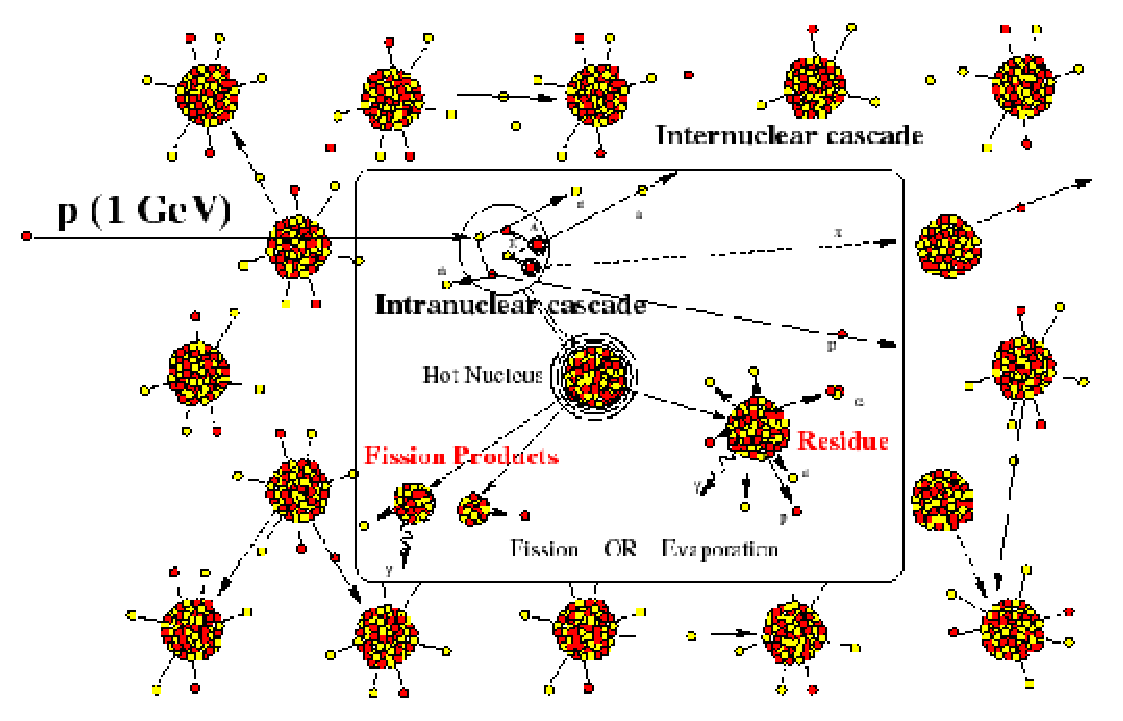
\includegraphics[scale=0.73]{images/cascade.eps}

%INCL is an intra-nuclear cascade model developed at the university of
%Li\`ege and CEA/Saclay.

%\end{textbox}
%%%%%%%%%%%%%%%%%%%%%%%%%%%%%%%%%%%%%%%%%%%%%%%%%%%%%%%%%%%%%%%%%%%%%%%%%%%%%%%
\begin{textbox}


\section*{{\Huge {\sf ABLA MODEL FOR EVAPO\-RATI\-ON AND FISSION}}}
%\section*{\color{udsect} ABLA}

ABLA is a fission and evaporation code that is developed at GSI, Darmstadt.

\end{textbox}
%%%%%%%%%%%%%%%%%%%%%%%%%%%%%%%%%%%%%%%%%%%%%%%%%%%%%%%%%%%%%%%%%%%%%%%%%%%%%%%%%
%\begin{textbox}


\section*{{\Huge {\sf p(1.2 GeV) + Pb $\rightarrow$ n + X}}}

Validating double-differential for neutron production from Geant4 INCL
and ABLA models. Evaporation from ABLA model is shown below E $\simeq$
20 MeV.

%\begin{figure}
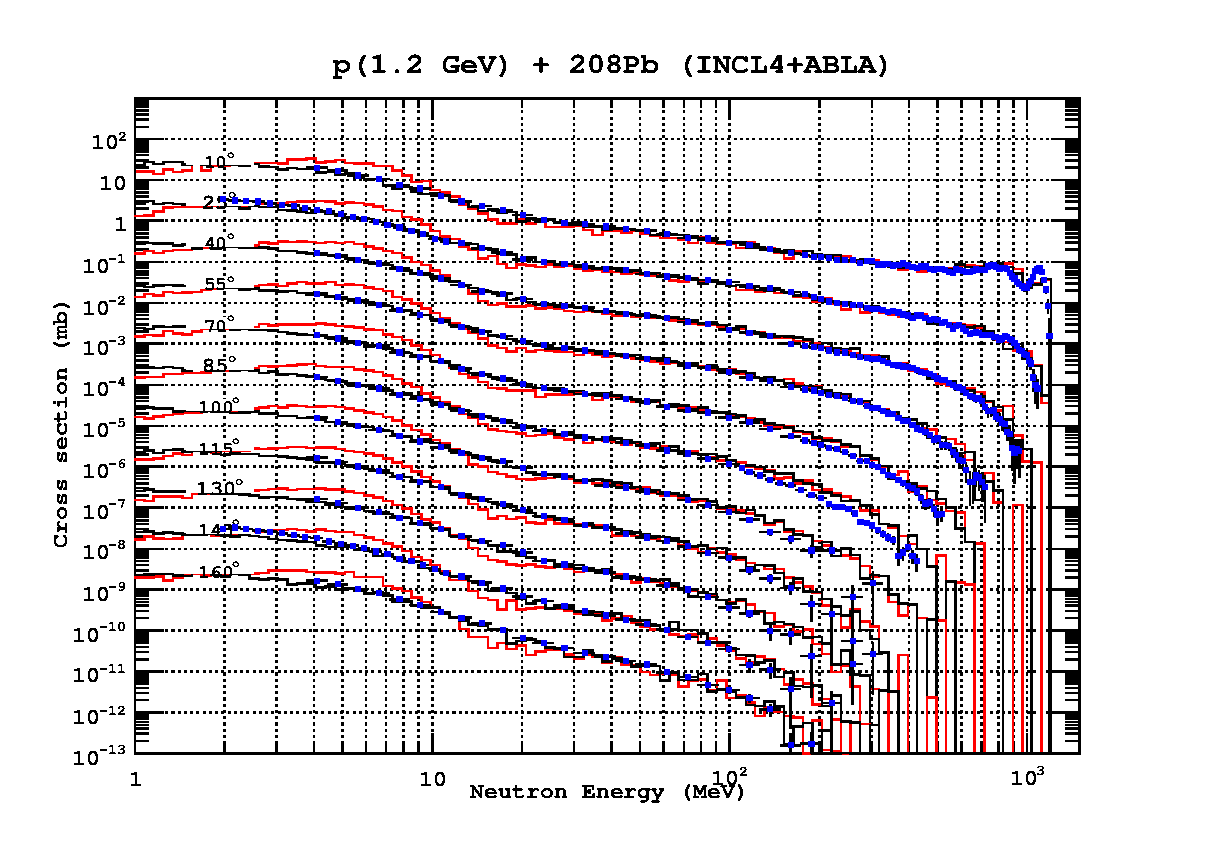
\includegraphics[scale=0.70]{images/pPbDD.eps}
%\label{fig:pPbdd1200MeV}
%\end{figure}

%\end{textbox}
%%%%%%%%%%%%%%%%%%%%%%%%%%%%%%%%%%%%%%%%%%%%%%%%%%%%%%%%%%%%%%%%%%%%%%%%%%%%%%%%%%
\begin{textbox}


\section*{{\Huge {\sf ABLA EVAPORATION}}}
The probabilities for emission of particle type $j = {p, n, \alpha}$
are calculated using formula:
\begin{equation}
W_j(N,Z,E) = \frac{\Gamma_j(N,Z,E)}{\sum_k\Gamma_k(N,Z,E)},
\label{eqn:probabilities}
\end{equation}
where $\Gamma_j$ is emission width for particle $j$, $N$ is neutron
number, $Z$ charge number and $E$ excitation energy.
\vskip0.5cm

Emission widths are calculated using the following formula:
\index{emission width}
\begin{equation}
\Gamma_j = \frac{1}{2 \pi \rho_c(E)} \frac{4 m_j R^2}{\hbar^2} T_j^2 \rho_j(E - S_j - B_j),
\label{eqn:emissionwidth}
\end{equation}
where:
\begin{itemize}
\item $\rho_c(E)$ and $\rho_j(E - S_j - B_j)$ are the level densities
of the compound nucleus and the exit channel, respectively.
\item $B_j$ is the height of the Coulomb barrier,
\item $S_j$ the separation energy,
\item $R$ is the radius,
\item $T_j$ the temperature of the remnant nucleus after
emission, and
\item $m_j$ the mass of the emitted particle.
\end{itemize}
\end{textbox}
%%%%%%%%%%%%%%%%%%%%%%%%%%%%%%%%%%%%%%%%%%%%%%%%%%%%%%%%%%%%%%%%%%%%%%%%%%%%%%%%%%

\section*{{\Huge {\sf }}}

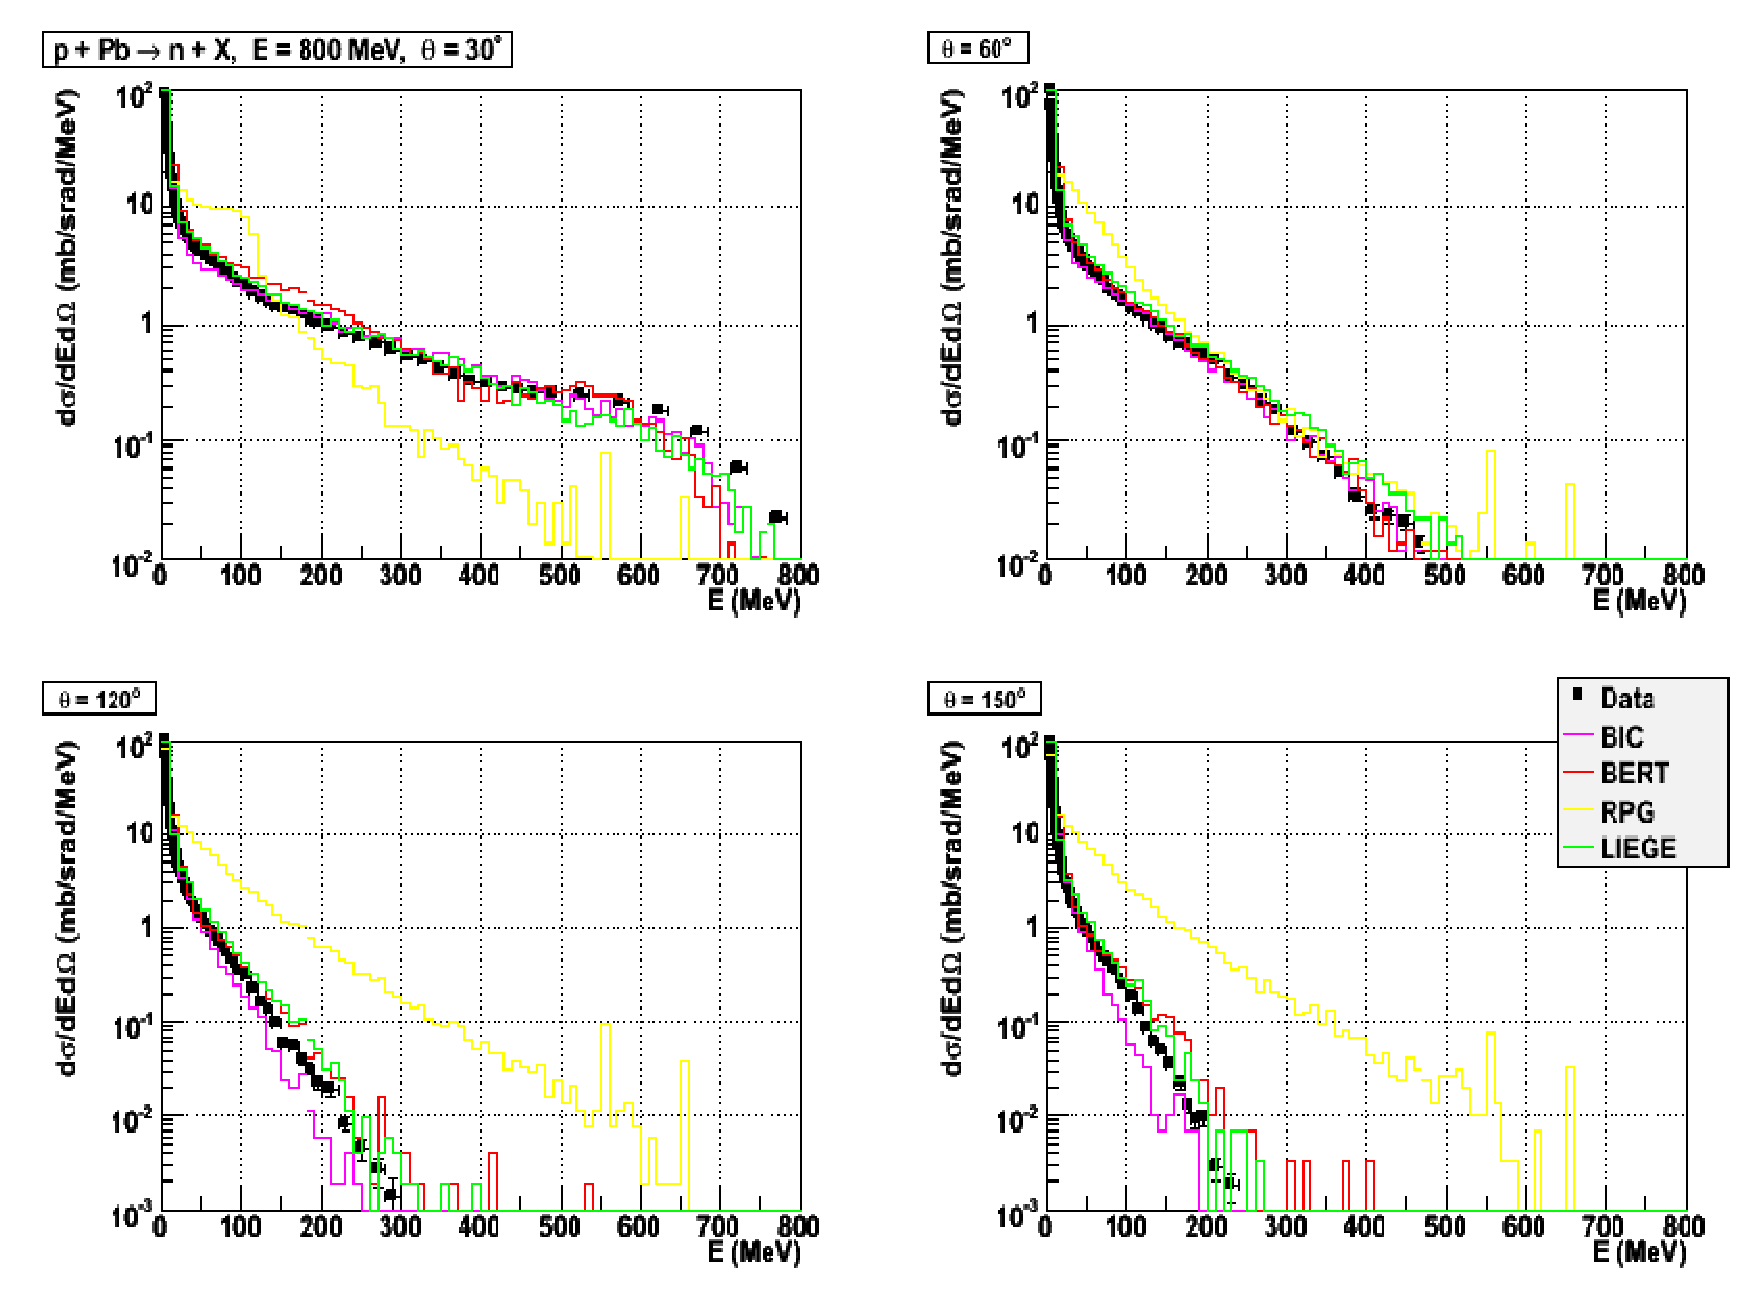
\includegraphics[scale=0.45]{images/vladimir.eps}
{\Large {\sf Comparison of various cascade models in Geant4. INCL/ABLA precision
model good agreement with experimental data. ({\emph Courtesy of
    V. Ivanchenko, Geant4 collaboration}).}}

%%%%%%%%%%%%%%%%%%%%%%%%%%%%%%%%%%%%%%%%%%%%%%%%%%%%%%%%%%%%%%%%%%%%%%%%%%%%%%%%%%%
\begin{textbox}


\section*{{\Huge {\sf ACKNOWLEDGEMENTS}}}

This work is a collaborative effort with the original developers from
Li\`ege University, GSI and CEA. We acknowledge the help from J. Cugnon,
A. Boudard, Y. Yariv, S. Leray, C. Schmidt and K. H. Schmidt.
converting the original FORTRAN codes C++ language.

\end{textbox}
%%%%%%%%%%%%%%%%%%%%%%%%%%%%%%%%%%%%%%%%%%%%%%%%%%%%%%%%%%%%%%%%%%%%%%%%%%%%%%%%%%%
\vskip2cm
\begin{textbox}

{\Large
\addcontentsline{toc}{section}{References}
\begin{thebibliography}{9}
\bibitem{incl} A. Boudard et al., \emph{Intranuclear cascade model for
    a comprehensive description of spallation reaction data}, Phys.
  Rev. C66 (2002) 044615
\bibitem{abla} J. Benlliure et al., \emph{Calculated nuclide
    production yields in relativistic collisions of fissile nuclei},
  Nuc. Phys. A628 (1998) 458
\bibitem{fp} P. Kaitaniemi, A. Heikkinen, \emph{Implementing INCL4
    hadronic cascade and ABLA de-excitation codes in Geant4},
  Proceedings of the 41th Annual Meeting of the Finnish Physical
  Society (2007)
\bibitem{g4} \emph{Geant4 collaboration website} {\tt http://\-cern.ch/\-geant4}
\bibitem{g4incl} \emph{Geant4 Physics Reference Manual: INCL 4.2 Cascade and ABLA V3 Evaporation with Fission} {\tt http://geant4.web.cern.ch/\-geant4/\-UserDocumentation/\-UsersGuides/\-PhysicsReferenceManual/\-html/\-node185.html}
%\bibliographystyle{abbrv}
%\bibliography{latex_poster}
\end{thebibliography}
}

\end{textbox}
%%%%%%%%%%%%%%%%%%%%%%%%%%%%%%%%%%%%%%%%%%%%%%%%%%%%%%%%%%%%%%%%%%%%%%%%%%%%%%%%%%%

\end{multicols}

\end{center}
\end{document}
